% Options for packages loaded elsewhere
\PassOptionsToPackage{unicode}{hyperref}
\PassOptionsToPackage{hyphens}{url}
%
\documentclass[
  12pt,
]{article}
\usepackage{lmodern}
\usepackage{amssymb,amsmath}
\usepackage{ifxetex,ifluatex}
\ifnum 0\ifxetex 1\fi\ifluatex 1\fi=0 % if pdftex
  \usepackage[T1]{fontenc}
  \usepackage[utf8]{inputenc}
  \usepackage{textcomp} % provide euro and other symbols
\else % if luatex or xetex
  \usepackage{unicode-math}
  \defaultfontfeatures{Scale=MatchLowercase}
  \defaultfontfeatures[\rmfamily]{Ligatures=TeX,Scale=1}
\fi
% Use upquote if available, for straight quotes in verbatim environments
\IfFileExists{upquote.sty}{\usepackage{upquote}}{}
\IfFileExists{microtype.sty}{% use microtype if available
  \usepackage[]{microtype}
  \UseMicrotypeSet[protrusion]{basicmath} % disable protrusion for tt fonts
}{}
\makeatletter
\@ifundefined{KOMAClassName}{% if non-KOMA class
  \IfFileExists{parskip.sty}{%
    \usepackage{parskip}
  }{% else
    \setlength{\parindent}{0pt}
    \setlength{\parskip}{6pt plus 2pt minus 1pt}}
}{% if KOMA class
  \KOMAoptions{parskip=half}}
\makeatother
\usepackage{xcolor}
\IfFileExists{xurl.sty}{\usepackage{xurl}}{} % add URL line breaks if available
\IfFileExists{bookmark.sty}{\usepackage{bookmark}}{\usepackage{hyperref}}
\hypersetup{
  pdftitle={Hurricane Michael and Floridian Turnout},
  pdfauthor={Kevin Morris; Peter Miller},
  hidelinks,
  pdfcreator={LaTeX via pandoc}}
\urlstyle{same} % disable monospaced font for URLs
\usepackage[margin=1in]{geometry}
\usepackage{longtable,booktabs}
% Correct order of tables after \paragraph or \subparagraph
\usepackage{etoolbox}
\makeatletter
\patchcmd\longtable{\par}{\if@noskipsec\mbox{}\fi\par}{}{}
\makeatother
% Allow footnotes in longtable head/foot
\IfFileExists{footnotehyper.sty}{\usepackage{footnotehyper}}{\usepackage{footnote}}
\makesavenoteenv{longtable}
\usepackage{graphicx}
\makeatletter
\def\maxwidth{\ifdim\Gin@nat@width>\linewidth\linewidth\else\Gin@nat@width\fi}
\def\maxheight{\ifdim\Gin@nat@height>\textheight\textheight\else\Gin@nat@height\fi}
\makeatother
% Scale images if necessary, so that they will not overflow the page
% margins by default, and it is still possible to overwrite the defaults
% using explicit options in \includegraphics[width, height, ...]{}
\setkeys{Gin}{width=\maxwidth,height=\maxheight,keepaspectratio}
% Set default figure placement to htbp
\makeatletter
\def\fps@figure{htbp}
\makeatother
\setlength{\emergencystretch}{3em} % prevent overfull lines
\providecommand{\tightlist}{%
  \setlength{\itemsep}{0pt}\setlength{\parskip}{0pt}}
\setcounter{secnumdepth}{5}
\usepackage{rotating}
\usepackage{setspace}
\newcommand{\beginsupplement}{\setcounter{table}{0}  \renewcommand{\thetable}{A\arabic{table}} \setcounter{figure}{0} \renewcommand{\thefigure}{A\arabic{figure}}}
\usepackage{booktabs}
\usepackage{longtable}
\usepackage{array}
\usepackage{multirow}
\usepackage{wrapfig}
\usepackage{float}
\usepackage{colortbl}
\usepackage{pdflscape}
\usepackage{tabu}
\usepackage{threeparttable}
\usepackage{threeparttablex}
\usepackage[normalem]{ulem}
\usepackage{makecell}
\usepackage{xcolor}
\newlength{\cslhangindent}
\setlength{\cslhangindent}{1.5em}
\newenvironment{cslreferences}%
  {\setlength{\parindent}{0pt}%
  \everypar{\setlength{\hangindent}{\cslhangindent}}\ignorespaces}%
  {\par}

\title{Hurricane Michael and Floridian Turnout\thanks{The authors thanks Many People for their comments on this project. All errors are our responsibility.}}
\author{Kevin Morris\footnote{Researcher, Brennan Center for Justice at NYU School of Law, 120 Broadway Ste 1750, New York, NY 10271 (\href{mailto:kevin.morris@nyu.edu}{\nolinkurl{kevin.morris@nyu.edu}})} \and Peter Miller\footnote{Researcher, Brennan Center for Justice at NYU School of Law, 120 Broadway Ste 1750, New York, NY 10271 (\href{mailto:peter.miller@nyu.edu}{\nolinkurl{peter.miller@nyu.edu}})}}
\date{October 07, 2020}

\begin{document}
\maketitle
\begin{abstract}
The United States is facing unprecedented challenges to election administration from the novel coronavirus. In response, many election administrators and advocates are calling for expanded vote-by-mail options to reduce in-person voting. To test the efficacy of loosened vote-by-mail rules we look to the experience of Florida in 2018, when Hurricane Michael devastated parts of the panhandle. By leveraging cross-jurisdiction variation in loosened restrictions in a double-matched triple-differences model, we show that loosened restrictions on vote-by-mail alone were not successful at eliminating administrative costs to voting. As administrators around the country loosen mail-voting restrictions in advance of this fall, they must couple these eased restrictions with strong public education campaigns about how voters can take advantange of them.
\end{abstract}

\pagenumbering{gobble}
\pagebreak

\pagenumbering{arabic}
\doublespacing

\hypertarget{research-design-and-expectations}{%
\section*{Research Design and Expectations}\label{research-design-and-expectations}}
\addcontentsline{toc}{section}{Research Design and Expectations}

We expect that Hurricane Michael depressed turnout in the 2018 midterm election via two causal mechanisms: individual-level effects, and administrative effects.

The hurricane likely directly reduced individual voters' propensity to vote. We know that Hurricane Michael caused substantial destruction; as discussed in the introduction to this paper, residents lost their lives, flooding was widespread, and the hurricane caused billions of dollars of property damage. Would-be voters were now faced with myriad disruptions to their daily lives; it is likely that the direct effects of the weather, therefore, reduced turnout substantially. As professor emeritus Robert Montjoy told NPR in the aftermath of the storm, ``Whether casting a ballot becomes a higher priority than cleaning out the basement, visiting someone in the hospital, or all the other demands\ldots You certainly expect a lower turnout for those reasons'' (Parks \protect\hyperlink{ref-Parks2018}{2018}).

The hurricane also caused problems for county election administrators, as the reporting around the Governor's executive order makes clear.\footnote{Executive Order 18-283 can be found here: \url{https://www.flgov.com/wp-content/uploads/2018/10/SLT-BIZHUB18101809500.pdf}.} Some mail voters\footnote{We use the terms mail and absentee voting interchangeably throughout this paper.} were residing in locations other than their registered addresses; would-be poll workers were unavailable; and the eight counties covered by the executive order collectively saw just 62 of the anticipated 127 polling places opened. Absent mitigation, the administrative effects of Hurricane Michael likely would have decreased turnout above-and-beyond the individual effects of the storm.

Executive Order 18-283 sought to offset the administrative barriers to voting by allowing county election administrators to flexibly respond to the damage wrought by the storm. Specifically, Executive Order 18-283 allowed administrators to add early voting locations; begin early voting 15 days before the general election, and continue until the day of the election; to accept vote-by-mail requests to addresses other than a voter's registered address; to send vote-by-mail ballots by forwardable mail; to deliver vote-by-mail ballots to electors or electors' immediate family members on election day without an affidavit; to relocate or consolidate polling places; and required poll watchers to be registered by the second Friday before the general election.

This paper sets out to answer a number of questions: what was the total depressive effect of the hurricane? Did Executive Order 18-283 effectively offset the depressive administrative effects? More specifically, did easing mail-balloting rules reduce the impact of closed polling places?

\hypertarget{estimating-the-net-effects-of-the-hurricane}{%
\subsection*{Estimating the Net Effects of the Hurricane}\label{estimating-the-net-effects-of-the-hurricane}}
\addcontentsline{toc}{subsection}{Estimating the Net Effects of the Hurricane}

We begin by testing the net effect of each of these treatments on individual-level turnout. Our central identification strategy involves the use of difference-in-differences models. We use voter-file data from L2 Political to estimate individual-level turnout and to control for individual-level characteristics. L2 uses models to predict individual race / ethnicity and voters' sex but these characteristics are available in self-reported form in the raw voter-file available from the state; as such, we pull sex and race / ethnicity from the publicly available voter file. The L2 data is based on the February 8, 2019, version of the raw voter file, the same file from which we pull race / ethnicity and sex.

By comparing historical and 2018 turnout for voters in the counties hit by the storm to historical and 2018 turnout of voters elsewhere in the state, we can estimate the effect of the storm on turnout. To ensure a high-quality difference-in-differences specification, we do not include all untreated voters in our control group; rather, we genetically match (Sekhon \protect\hyperlink{ref-Sekhon2011}{2011}) each treated voter with five untreated voters along a battery of individual- and neighborhood-level characteristics. Untreated voters who do not serve as matches are excluded from our models. Although it may seem counterintuitive to exclude data from our models, this matching procedure substantially improves the parallel trends assumptions necessary for a rigorous difference-in-differences analysis.

This design allows us to test our first hypothesis:

\textbf{Hypothesis 1:} Turnout among voters in the eight treated counties was depressed in the 2018 election relative to voters in untreated counties. This represents the net effect of both the individual and administrative level treatments.

\hypertarget{decomposing-individual-and-administrative-effects}{%
\subsection*{Decomposing Individual and Administrative Effects}\label{decomposing-individual-and-administrative-effects}}
\addcontentsline{toc}{subsection}{Decomposing Individual and Administrative Effects}

To estimate the administrative effect on turnout, we must control for the individual-level effects of the storm. To do so, we leverage the somewhat arbitrary borders of counties in the Florida Panhandle. There is no reason to believe that the effects of a hurricane would change dramatically along county borders. We assume, therefore, that voters who lived nearby one another, but on either side of a county border, faced the same weather issues during the 2018 election. In other words, they were subject to the same individual-level treatments. We assume that voters on either side of these administrative boundaries are comparable. Any observed turnout differentials, therefore, can be explained by the county in which they happen to live. Put differently, any turnout differential between votes in the eight treated counties and voters just outside these counties is the administrative effect of the hurricane on turnout in the treated counties. Walker, Herron, and Smith (\protect\hyperlink{ref-Walker2019}{2019}) similarly leverages county borders to identify the causal effect of county-specific circumstances on turnout.

To disaggregate the individual and administrative effects of Hurricane Michael, we employ a double-matched triple-differences (or difference-in-difference-in-differences) specification.

We begin by constructing our set of treated voters. These treated voters include all registered voters who live in a treated county and within 2.5 miles of a bordering, untreated county (See Figure \ref{fig:map}). Each treated voter is then each matched to one voter who lives in an untreated county, but within 2.5 miles of a treated county. These matches are considered primary control voters. They were subject to identical \emph{individual} level treatments as the treated voters, but different \emph{administrative} treatments.

Each treated and primary control voter is subsequently matched to five voters elsewhere in the state --- that is to say, voters who are neither in the treated counties nor in the counties directly surrounding the treated counties. This exercise is the second match, and the matches are our ``secondary control voters.'' These voters were subject to neither individual-level nor administrative-level treatments.

At this point, we have three distinct groups of voters:

\begin{itemize}
\tightlist
\item
  Treated voters. These voters were subject to individual- and administrative-level effects from Hurricane Michael
\item
  Primary control voters. These voters were subject to individual, but not administrative, effects from Hurricane Michael.
\item
  Secondary control voters. These voters were subject to neither individual nor administrative effects.
\end{itemize}

Having constructed our pool of voters, we run a triple-differences model. This triple-differences model is, in effect, two simultaneous difference-in-differences models. The model estimates whether 2018 was associated with depressed turnout for our primary control voters vis-à-vis their controls. Because these primary control voters lived in counties not covered by the executive order, we assume that they faced no administrative effects from the storm. Any observed difference between these groups is therefore the individual-level effect of the storm for treated and primary control voters.

The model also estimates turnout differences between treated and primary control voters. Because the only difference between treated and primary control voters is the administrative district in which they lived, this estimated difference is interpreted as the administrative effect on turnout in the treated counties.

The double-matched triple-differences model allows us to test our second and third hypotheses:

\textbf{Hypothesis 2:} We expect that the hurricane had negative individual-level effects for voters who lived just outside of treated counties.

\textbf{Hypothesis 3:} We expect that the administrative effects of Hurricane Michael were negative, notwithstanding Executive Order 18-283.

After estimating the double-matched triple-differences model, we turn to vote-mode within the treated counties. We submitted public records requests to each of the eight counties covered by the executive order requesting the planned and actual location of each polling place. Two counties --- Calhoun and Liberty --- were able to use all of their expected polling places. Others were either forced to relocate or consolidate polling places. Most notably, Bay County went from an expected 44 polling places to just six.

To estimate the efficacy of mail-voting within the treated counties, we begin by calculating how far each voter lived from her closest planned polling place, and how far she lived from the closest polling place that was actually open on election day. Using the registered voter file, we can tell not only \emph{whether} a voter participated, but also \emph{how} they participated. Using a multinomial logistic regression, we test whether the difference between the planned and actual distance-to-polling-place were associated with vote-mode in 2018. This specification allows us to test our final hypothesis:

\textbf{Hypothesis 4}: As the difference between the actual and planned distance to the closest polling place increased for voters, they were more likely to vote absentee and to abstain from voting, relative to past behavior, all else being held equal.

\hypertarget{results}{%
\section*{Results}\label{results}}
\addcontentsline{toc}{section}{Results}

\hypertarget{overall-turnout-effects}{%
\subsection*{Overall Turnout Effects}\label{overall-turnout-effects}}
\addcontentsline{toc}{subsection}{Overall Turnout Effects}

We begin by matching each registered voter in the eight treated counties to five untreated voters elsewhere in the state using a genetic matching algorithm (Sekhon \protect\hyperlink{ref-Sekhon2011}{2011}).\footnote{Due to computing constraints, the matching weights were constructed using a one percent random sample stratified by treatment status.} The individual-level characteristics come directly from the registered voter file. The two neighborhood-level characteristics included --- median income and share of the population with some collegiate education --- are estimated at the block group level, and come from the ACS 5-year estimates ending with 2018. Ties are not broken, which means that some treated voters are assigned more than five control voters; the weights used in the regressions below are adjusted accordingly.

Although the treated counties were the at the center of the storm, nearby counties might have also been negatively impacted by the storm. Therefore, voters who live in the counties that border the treated counties are excluded. These include Walton, Holmes, Wakulla, and Leon Counties.

Table \ref{tab:full-bal} demonstrates the results of this matching procedure. As Table \ref{tab:full-bal} makes clear, voters in the affected counties were considerably more likely to be white and identify as Republicans, and live in lower-income neighborhoods, than voters in the rest of the state. The post-match control group, however, looks substantially similar to the treated voters.

\begin{singlespace}
\begin{table}[H]

\caption{\label{tab:balance-tab-full}\label{tab:full-bal} Balance Table for Statewide Matching}
\centering
\resizebox{\linewidth}{!}{
\begin{tabular}[t]{lllllrrrr}
\toprule
\multicolumn{1}{c}{ } & \multicolumn{2}{c}{Means: Unmatched Data} & \multicolumn{2}{c}{Means: Matched Data} & \multicolumn{4}{c}{Percent Improvement} \\
\cmidrule(l{3pt}r{3pt}){2-3} \cmidrule(l{3pt}r{3pt}){4-5} \cmidrule(l{3pt}r{3pt}){6-9}
 & Treated & Control & Treated & Control & Mean Diff & eQQ Med & eQQ Mean & eQQ Max\\
\midrule
\%White & 76.5\% & 62.3\% & 76.5\% & 76.5\% & 100.00 & 100.00 & 100.00 & 100.00\\
\% Black & 17.1\% & 13.1\% & 17.1\% & 17.1\% & 100.00 & 100.00 & 100.00 & 100.00\\
\% Latino & 2.1\% & 17.4\% & 2.1\% & 2.1\% & 100.00 & 100.00 & 100.00 & 100.00\\
\% Asian & 1.0\% & 2.0\% & 1.0\% & 1.0\% & 100.00 & 100.00 & 100.00 & 100.00\\
\% Female & 52.5\% & 52.4\% & 52.5\% & 52.5\% & 100.00 & 100.00 & 100.00 & 100.00\\
\% Male & 45.8\% & 44.9\% & 45.8\% & 45.8\% & 100.00 & 100.00 & 100.00 & 100.00\\
Age & 52.232 & 52.489 & 52.232 & 52.229 & 98.54 & 96.68 & 97.36 & 96.17\\
\% Democrat & 39.2\% & 37.1\% & 39.2\% & 39.2\% & 100.00 & 100.00 & 100.00 & 100.00\\
\% Republican & 43.6\% & 35.0\% & 43.6\% & 43.6\% & 100.00 & 100.00 & 100.00 & 100.00\\
\% with Some College & 69.0\% & 75.1\% & 69.0\% & 69.0\% & 99.77 & 99.00 & 98.05 & 88.66\\
Median Income & \$50,643 & \$62,941 & \$50,643 & \$50,654 & 99.91 & 98.11 & 96.89 & 86.56\\
\bottomrule
\end{tabular}}
\end{table}
\end{singlespace}

Figure \ref{fig:full-to} plots the turnout in the past few elections for our treated and control voters. As Figure \ref{fig:full-to} makes clear, treated voters consistently turned out at higher rates than control voters from 2010 -- 2016. In 2018, however, this relationship was inverted as turnout among treated voters plummeted from its 2016 level. Although turnout among all voters was higher in 2018 than in 2014, turnout rose by substantially less for the treated voters.

\begin{figure}[H]

{\centering 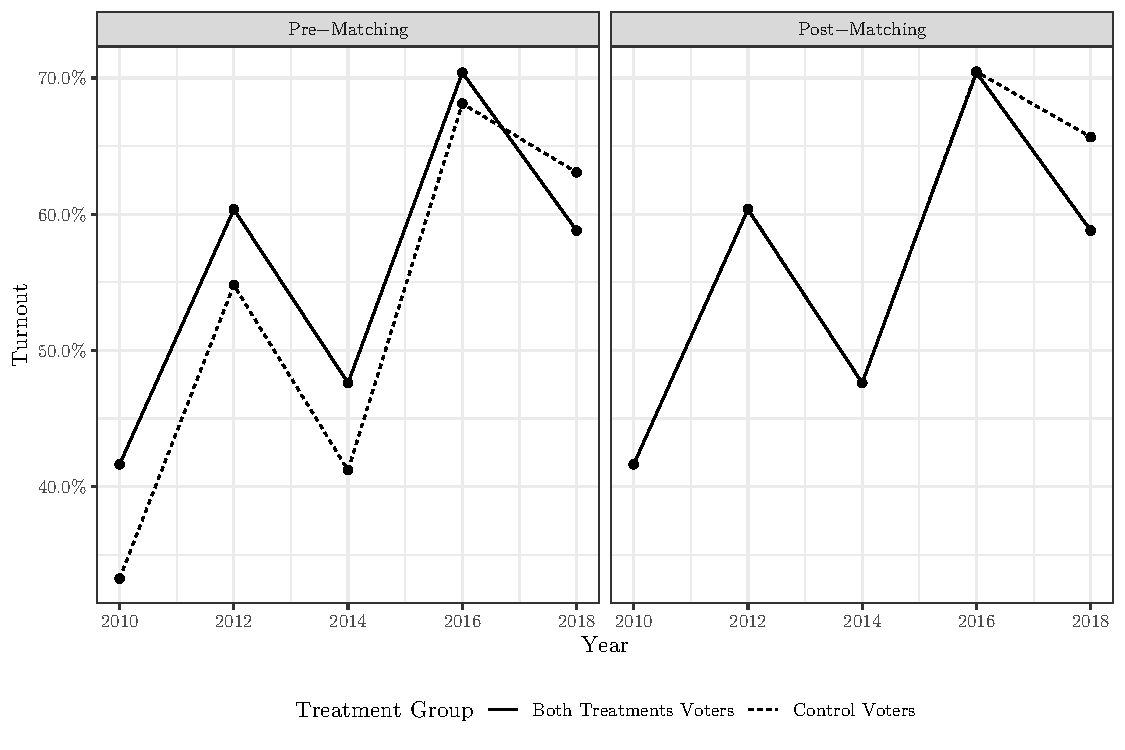
\includegraphics{hurricane_michael_files/figure-latex/full-to-chunk-1} 

}

\caption{\label{fig:full-to}General Election Turnout for Treated and Control Voters, 2010 -- 2018}\label{fig:full-to-chunk}
\end{figure}

Table \ref{tab:full-dind} formalizes Figure \ref{fig:full-to} into a differences-in-differences regression specification. We employ an ordinary least squares specification. The dependent variable takes the value 1 if a voter cast a ballot in a given year, and 0 if she did not. In each model, \emph{Treated × 2018} estimates the casual (net) effect of Hurricane Michael on turnout for treated voters. Model 2 also includes the characteristics on which the voters were matched. Model 3, finally, adds a measure for congressional district competitiveness. Because this variable is ``downstream'' of treatment --- that is to say, the effect of the hurricane could have impacted the competitiveness of certain races --- it is not included in the first two models. It should be noted that each of the treated voters lived in uncontested congressional districts. Robust standard errors are clustered at the level of the match (Abadie and Spiess \protect\hyperlink{ref-Abadie2019}{2019}).

\begin{singlespace}
\input{"../temp/dind_full.tex"}
\end{singlespace}

The coefficient on \emph{Treated × 2018} in Table \ref{tab:full-dind} indicates that Hurricane Michael had a substantial depressive effect in 2018 among the treated voters. Each model estimates that the overall effect --- including individual and administrative effects --- was -9.4 percentage points. Multiplied across the nearly 200 thousand registered voters in the treated counties indicates that some 19 thousand ballots went uncast due to the hurricane --- a major effect in a year when a statewide senate race was decided by 10,033 votes.

\hypertarget{identifying-administrative-effects}{%
\subsection*{Identifying Administrative Effects}\label{identifying-administrative-effects}}
\addcontentsline{toc}{subsection}{Identifying Administrative Effects}

As discussed above, our primary strategy for isolating the administrative effects of the hurricane on turnout involves leveraging random assignment around county borders in the Florida panhandle in a double-matched triple-differences specification.

We begin by identifying all voters who lived within 2.5 miles of a county with a different treatment status. Figure \ref{fig:map} shows the map of counties in the region. The eight treated counties are drawn in a medium gray, and the untreated border counties are drawn in dark gray. All treated and control voters come from the light gray buffer, which extends for 2.5 miles on either side of the border between a treated and untreated county. There are not voters in Gulf, Calhoun, or Franklin Counties who live within 2.5 miles of an untreated county.

\begin{figure}[H]

{\centering 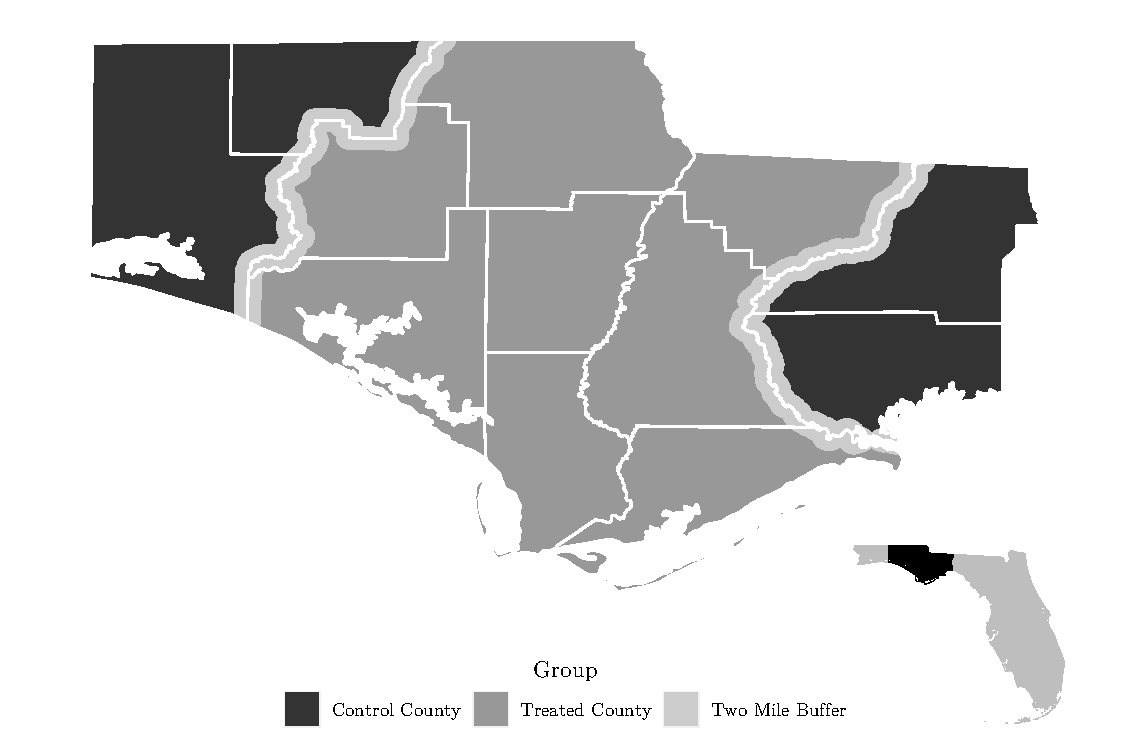
\includegraphics{hurricane_michael_files/figure-latex/map-chunk-1} 

}

\caption{\label{fig:map}Treated and Control Counties with 2.5 Mile Buffer}\label{fig:map-chunk}
\end{figure}

Each voter inside the buffer in a treated county is matched with one voter in the buffer in an untreated county, once again using a genetic matching algorithm (Sekhon \protect\hyperlink{ref-Sekhon2011}{2011}). These matches serve as our primary control voters. Ties are not broken, which means that some treated voters are assigned multiple primary control voters; the weights used in the regressions are adjusted accordingly.

In some cases, voters on either side of the border are in different congressional districts. This would pose a problem if these races were contested thanks to the potentially mobilizing effects of house races, but the entire buffer falls in uncontested congressional districts. This means that treated and untreated voters are not facing differential mobilization from congressional races. As before, we match on individual- and neighborhood-level characteristics. Importantly, we match treated and untreated voters using their latitude and longitude to ensure that matches live in close proximity to one another. Table \ref{tab:balance-ll} presents the results of this matching exercise.

\begin{singlespace}
\begin{table}[H]

\caption{\label{tab:balance-tab-ll}\label{tab:balance-ll} Balance Table for Border Buffer Matching}
\centering
\resizebox{\linewidth}{!}{
\begin{tabular}[t]{lllllrrrr}
\toprule
\multicolumn{1}{c}{ } & \multicolumn{2}{c}{Means: Unmatched Data} & \multicolumn{2}{c}{Means: Matched Data} & \multicolumn{4}{c}{Percent Improvement} \\
\cmidrule(l{3pt}r{3pt}){2-3} \cmidrule(l{3pt}r{3pt}){4-5} \cmidrule(l{3pt}r{3pt}){6-9}
 & Treated & Control & Treated & Control & Mean Diff & eQQ Med & eQQ Mean & eQQ Max\\
\midrule
\%White & 71.2\% & 74.9\% & 71.2\% & 71.2\% & 100.00 & 100.00 & 100.00 & 100.00\\
\% Black & 24.8\% & 18.2\% & 24.8\% & 24.7\% & 98.65 & 98.66 & 98.66 & 98.66\\
\% Latino & 1.1\% & 2.3\% & 1.1\% & 1.1\% & 100.00 & 100.00 & 100.00 & 100.00\\
\% Asian & 0.3\% & 0.8\% & 0.3\% & 0.3\% & 100.00 & 100.00 & 100.00 & 100.00\\
\% Female & 53.2\% & 53.0\% & 53.2\% & 53.2\% & 100.00 & 100.00 & 100.00 & 100.00\\
\% Male & 45.4\% & 45.1\% & 45.4\% & 45.4\% & 100.00 & 100.00 & 100.00 & 100.00\\
Age & 53.139 & 50.197 & 53.139 & 53.097 & 98.58 & 87.44 & 86.74 & 81.79\\
\% Democrat & 47.2\% & 44.5\% & 47.2\% & 47.2\% & 97.59 & 97.60 & 97.60 & 97.60\\
\% Republican & 39.1\% & 37.7\% & 39.1\% & 39.1\% & 100.00 & 100.00 & 100.00 & 100.00\\
\% with Some College & 62.7\% & 70.0\% & 62.7\% & 63.0\% & 95.63 & 63.99 & 62.43 & 59.15\\
Median Income & \$45,243 & \$51,335 & \$45,243 & \$46,004 & 87.50 & -12.08 & 43.03 & 46.56\\
\bottomrule
\end{tabular}}
\end{table}
\end{singlespace}

The match procedure improves the balance between treated and primary control voters substantially for 10 of the 11 characteristics listed in Table \ref{tab:balance-ll}. The share Latino --- the only characteristic to go unimproved --- is below 2 percent for both groups and the difference is unlikely to cause any problems. Although latitudes and longitudes are not displayed in the table, the average treated voter lives 9.5 miles from her primary control voter.

Once our set of treated and primary control voters has been identified, each of these voters is matched with five other voters that lived in neither the treated nor the immediately surrounding counties. For ease of notation, the combined set of treated and primary control voters will henceforth be referred to as ``Panhandle voters,'' while ``treated'' voters will distinguish Panhandle voters in treated counties from Panhandle voters in other counties. The use of ``Panhandle'' is a slight misnomer: it excludes Escambia, Santa Rosa, and Okaloosa Counties which are certainly part of the Florida Panhandle, as well as Jefferson County and others to its east which are sometimes considered part of the panhandle. Nevertheless, we adopt this shorthand for referring to the treated counties and their neighbors.

This matching procedure follows the same steps detailed in the Overall Turnout Effects section of this paper. Table \ref{tab:balance-secondary} presents the results of the secondary match. We improve along all characteristics.

\begin{singlespace}
\begin{table}[H]

\caption{\label{tab:balance-tab-ll2}\label{tab:balance-secondary} Balance Table for Secondary Match}
\centering
\resizebox{\linewidth}{!}{
\begin{tabular}[t]{lllllrrrr}
\toprule
\multicolumn{1}{c}{ } & \multicolumn{2}{c}{Means: Unmatched Data} & \multicolumn{2}{c}{Means: Matched Data} & \multicolumn{4}{c}{Percent Improvement} \\
\cmidrule(l{3pt}r{3pt}){2-3} \cmidrule(l{3pt}r{3pt}){4-5} \cmidrule(l{3pt}r{3pt}){6-9}
 & Treated & Control & Treated & Control & Mean Diff & eQQ Med & eQQ Mean & eQQ Max\\
\midrule
\%White & 71.7\% & 62.3\% & 71.7\% & 71.7\% & 100.00 & 100.00 & 100.00 & 100.00\\
\% Black & 23.3\% & 13.1\% & 23.3\% & 23.3\% & 100.00 & 100.00 & 100.00 & 100.00\\
\% Latino & 1.4\% & 17.4\% & 1.4\% & 1.4\% & 100.00 & 100.00 & 100.00 & 100.00\\
\% Asian & 0.5\% & 2.0\% & 0.5\% & 0.5\% & 100.00 & 100.00 & 100.00 & 100.00\\
\% Female & 52.7\% & 52.4\% & 52.7\% & 52.7\% & 100.00 & 100.00 & 100.00 & 100.00\\
\% Male & 45.6\% & 44.9\% & 45.6\% & 45.6\% & 100.00 & 100.00 & 100.00 & 100.00\\
Age & 52.891 & 52.489 & 52.891 & 52.884 & 98.12 & 82.32 & 87.10 & 87.22\\
\% Democrat & 46.4\% & 37.1\% & 46.4\% & 46.4\% & 100.00 & 100.00 & 100.00 & 100.00\\
\% Republican & 38.7\% & 35.0\% & 38.7\% & 38.7\% & 100.00 & 100.00 & 100.00 & 100.00\\
\% with Some College & 62.9\% & 75.1\% & 62.9\% & 62.9\% & 99.98 & 99.30 & 97.16 & 82.78\\
Median Income & \$45,913 & \$62,941 & \$45,913 & \$45,928 & 99.91 & 99.03 & 96.22 & 80.63\\
\bottomrule
\end{tabular}}
\end{table}
\end{singlespace}

In Figure \ref{fig:trip-diff-plot} we present the plotted turnout trends from the treatment, primary control, and secondary control groups returned by the matching exercise. Figure \ref{fig:trip-diff-plot} makes clear that the turnout gap in these groups was relatively constant prior to 2018 (after accounting for differences in midterm and presidential elections), but that the relative turnout of the treatment group --- whose turnout in midterm elections was historically higher than the other groups --- noticeably dipped in 2018.

\begin{figure}[H]

{\centering 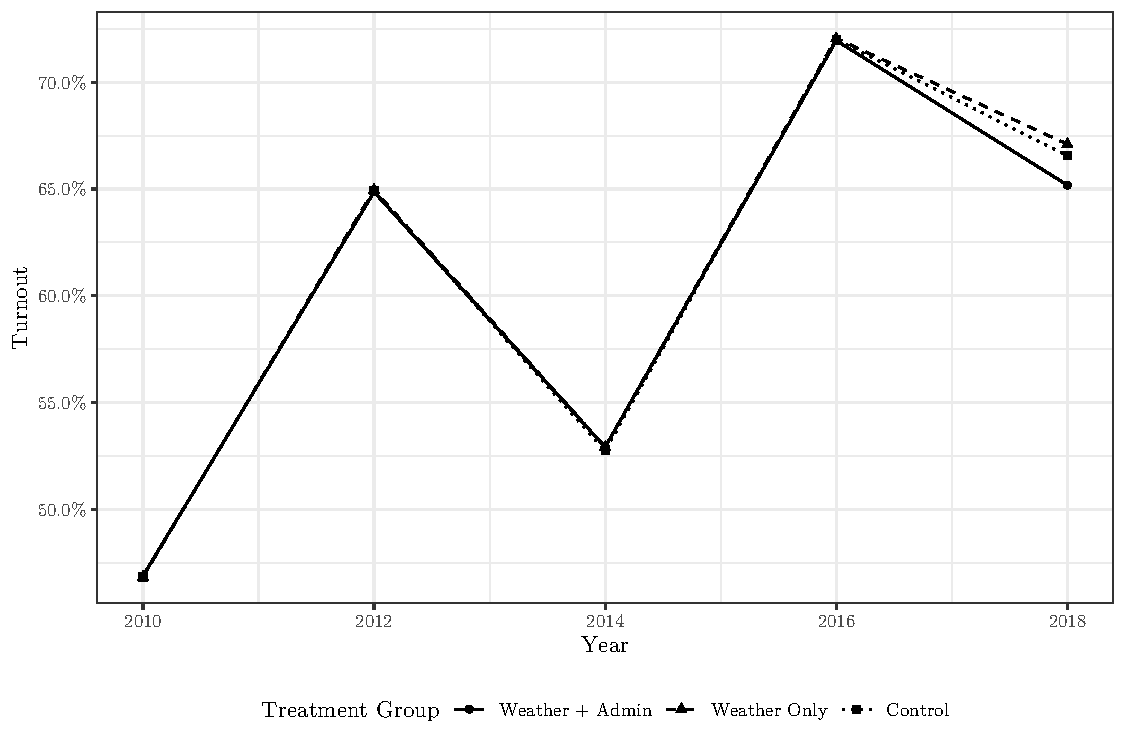
\includegraphics{hurricane_michael_files/figure-latex/tripd-to-chunk-1} 

}

\caption{\label{fig:trip-diff-plot}General Election Turnout for Treated, Primary Control, and Secondary Control Voters, 2010 -- 2018}\label{fig:tripd-to-chunk}
\end{figure}

Disentangling the administrative and individual effects of the storm requires the estimation of the triple-differences model. This model is estimated by Equation (1).

\begin{gather}
\label{eq:1}
v_{it}=\beta_0+\beta_1Panhandle_{i}+\beta_22018_{t}+\beta_3Panhandle_{i}\times 2018_{t} + \nonumber \\
\beta_4Treated_{i} + \beta_5Treated_{i}\times 2018_{t} + \beta_6Secondary Control Group 1_{i} + \\
\beta_7Midterm_{t} + \beta_8Panhandle_{i}\times Midterm_{t} + \beta_9Treated_{i}\times Midterm_{t} + \nonumber \\
\delta{Z}_{i} + \mathcal{E}_{it}. \nonumber
\end{gather}

Individual \emph{i}'s turnout (\emph{v}) in year \emph{t} is a function of the year and their location. In the equation, \emph{b\textsubscript{1}Pandhandle\textsubscript{i}} measures the historical difference between voters in the panhandle (both treated and matched, untreated individuals) and the rest of the state. \emph{b\textsubscript{2}2018\textsubscript{t}} measures the statewide change in turnout in 2018 from the baseline, while \emph{b\textsubscript{3}Panhandle\textsubscript{i} × 2018\textsubscript{t}} tests whether turnout changed differently in 2018 in the panhandle than it did elsewhere. \emph{b\textsubscript{3}Panhandle\textsubscript{i} × 2018\textsubscript{t}}, therefore, is our estimation of the individual-level, or weather related, effect of the hurricane. \emph{b\textsubscript{4}Treated\textsubscript{i}} measures the historical difference between treated and control observations in the buffer, and \emph{b\textsubscript{5}Treated\textsubscript{i} × 2018\textsubscript{t}} tests whether the change in turnout in 2018 was different for voters living in the treated counties than for their matched controls in the panhandle. We also test whether the secondary control voters for the treatment group had higher or lower turnout than the other set of secondary control voters using \emph{b\textsubscript{6}SecondaryControlGroup1\textsubscript{i}} term.

Figure \ref{fig:trip-diff-plot} indicates that there are different gaps between groups of voters in midterm and presidential years. These baseline differences are captured in the variables \emph{b\textsubscript{7}Midterm\textsubscript{t}}, \emph{b\textsubscript{8}Panhandle\textsubscript{i} × Midterm\textsubscript{t}}, and \emph{b\textsubscript{9}Treated\textsubscript{i} × Midterm\textsubscript{t}}. Finally, the matrix \emph{\(\delta\)Z\textsubscript{i}} contains the individual- and neighborhood-level characteristics on which the match was performed, included in some of the models.

Table \ref{tab:trip-diff} presents the results of this model, again fit using an ordinary least squares specification. Model 1 includes only the dummies discussed above, while Model 2 includes all the covariates on which the matching procedures were performed. Model 3 also includes estimates for congressional district competitiveness in 2018. Robust standard errors are clustered at the level of the original treated voter from which the primary and secondary controls arise.

\begin{singlespace}

\input{"../temp/triple_diff.tex"}
\end{singlespace}

The coefficients on \emph{Panhandle × 2018} and \emph{Treated × 2018} are of most substantive interest here. The coefficient on \emph{Panhandle × 2018} indicates that turnout for the primary control voters in 2018 was -3.8 percentage points below that of the secondary controls. Put differently, the individual-level effect of the storm on treated and primary control voters was -3.8 points.

\emph{Treated × 2018} indicates that, for voters just inside the treated counties, turnout was depressed by an \emph{additional} 3.1 percentage points. This 3.1 percentage point decrease in turnout for voters inside the treated counties is the administrative effect on turnout. Taken as a whole, the net effect of the hurricane on voters just inside the treatment counties was therefore -6.9 percentage points.

Importantly, the decomposed administrative- and individual- effects estimated in Table \ref{tab:trip-diff} are the average treatment effect on the treated voters (ATT). These models include only treated voters at the very edges of the hardest-hit counties, and it is therefore unsurprising that the net effect estimated by the triple-differences models are smaller than the net effects estimated in Table \ref{tab:full-to}, where all voters in the 8 treated counties are included. Nevertheless, the administrative effect of -3.1 percentage points is substantively quite large. Despite the efforts of Executive Order 18-283, the administrative hurdles posed by Hurricane Michael meaningfully depressed turnout.

\hypertarget{where-did-the-ballots-go}{%
\section*{Where Did the Ballots Go?}\label{where-did-the-ballots-go}}
\addcontentsline{toc}{section}{Where Did the Ballots Go?}

Having established that turnout was substantially depressed in the treated counties and that a non-trivial amount of the depression arose from administrative costs, we turn to a new question: where did these ballots go? We know that Executive Order 18-283 loosened restrictions on early and mail balloting; we therefore expect that, relative to the rest of the state, a higher share of ballots in the treated counties cast their ballots in one of these ways.

We return to the matches produced earlier in this paper, where every voter in the treated counties was matched with five voters elsewhere in the state. Figure \ref{fig:vote-mode} demonstrates the share of registered voters that cast a ballot either at the polling place, early in person, or absentee. In each case, the denominator is the number of registered voters in 2018.

\begin{figure}[H]

{\centering 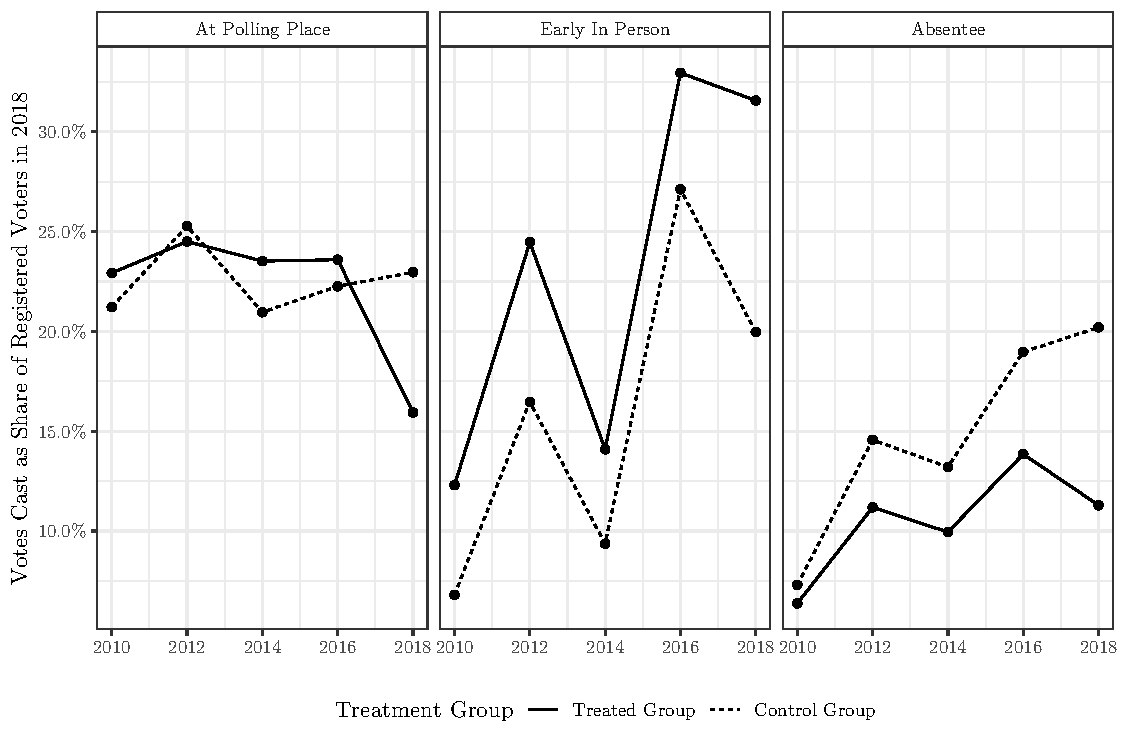
\includegraphics{hurricane_michael_files/figure-latex/vote-mode-chunk-1} 

}

\caption{\label{fig:vote-mode}Marginal Effect of Relocated Polling Place on Vote Mode}\label{fig:vote-mode-chunk}
\end{figure}

Figure \ref{fig:vote-mode} makes clear that the decline in turnout was a product of lower turnout on election day, and perhaps via absentee voting. It is possible, however, that early voting was actually higher in the treated counties due to Hurricane Michael. These plots, however, are somewhat noisy. As such, we refrain from estimating difference-in-differences models, as the parallel trends assumption seems to be violated by the historical data. Nevertheless, Figure \ref{fig:vote-mode} provides some evidence of how Hurricane Michael shifted vote methods.

To more directly estimate the effect of Hurricane Michael and the closing of polling places on vote-mode, we measure the distance between each voter in the treated counties and the closest planned polling place, and the closest polling place actually open on election day. Using a multinomial logistic regression, we test whether increasing the difference between this distance is related to vote-mode or abstention in 2018. Table \ref{tab:treated-multi} presents the result of this specification, where each option is measured relative to in-person election day voting. In addition to the difference between expected and actual distance to the closest polling place (\emph{Change in Distance to Polling Place (km)}), we include other covariates. \emph{Distance to Closest Planned Polling Place (km)} measures how far a voter lived from her closest planned polling place, in case voters in more remote parts of the counties generally voted differently in 2018 than other voters. We include other covariates for individual characteristics such as race, age, and partisan affiliation. We also include dummies indicating how (or whether) each voter participated in the 2012 -- 2016 general elections. The logistic coefficients are transformed into relative risk ratios (standard errors are left untransformed).

\begin{singlespace}
\input{"../temp/multinom.tex"}
\end{singlespace}

Table \ref{tab:treated-multi} indicates that for each additional kilometer a voter had to travel above-and-beyond the distance to her planned polling place, she was more likely to vote early, to vote by mail, and to abstain altogether than vote in-person on election day. Although these are each statistically significant at the 99 percent level, an examination of the marginal effects plots indicates that their relative importance differed substantially. Figure \ref{fig:marg-multi} presents the marginal effect of the change in distance to the nearest polling place on vote method while keeping all other covariates in Table \ref{tab:treated-multi} at their means.

\begin{figure}[H]

{\centering 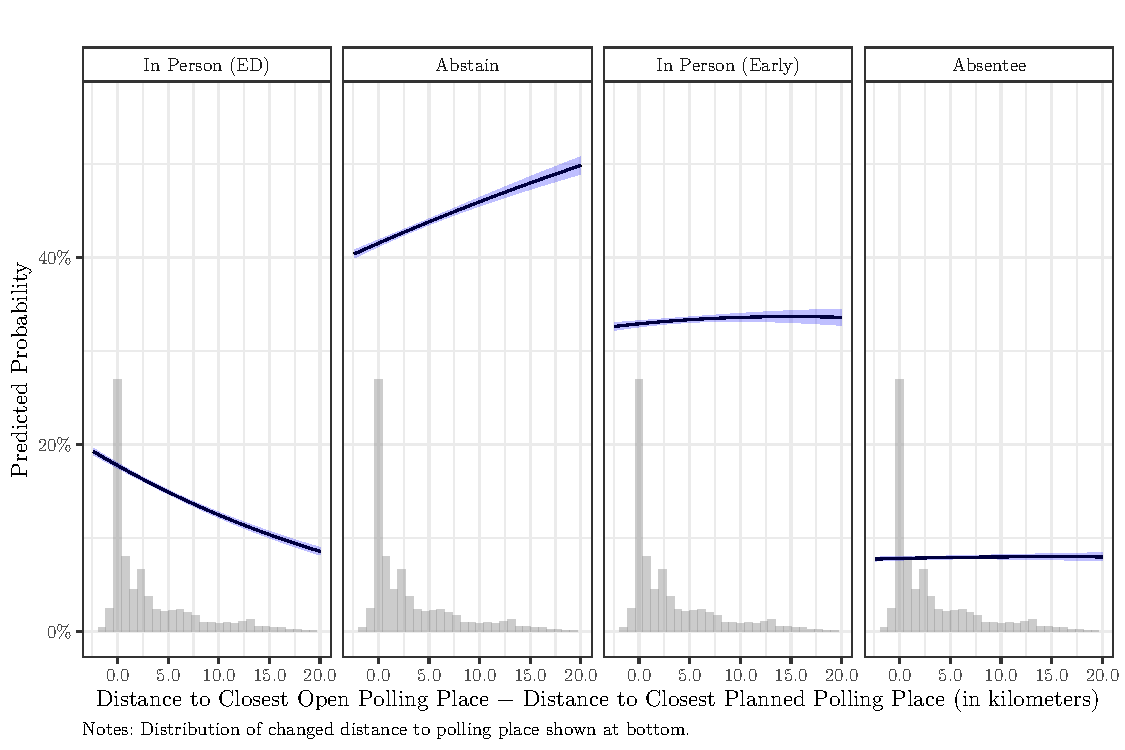
\includegraphics{hurricane_michael_files/figure-latex/marg-multi-1} 

}

\caption{\label{fig:marg-multi}Marginal Effect of Changed Distance to Polling Place on 2018 Vote Mode}\label{fig:marg-multi}
\end{figure}

Figure \ref{fig:marg-multi} indicates that, as voters suddenly had to travel further to the nearest polling place, they were substantially less likely to vote in-person on election day. The bulk of these voters \emph{did not} shift to absentee voting or early in-person voting; rather, they were much more likely to abstain from casting a ballot at all. Thus, although administrators took steps to make early and mail voting easier, these efforts were not particularly effective.

\hypertarget{discussion-and-conclusion}{%
\section*{Discussion and Conclusion}\label{discussion-and-conclusion}}
\addcontentsline{toc}{section}{Discussion and Conclusion}

Election Day in the United States consistently falls near the end of hurricane season. Hurricane Michael made landfall on October 10, 2018, less than a month before the highest-turnout midterm election in a century. Superstorm Sandy struck New York and New Jersey just days before the midterm elections in 2012, wreaking immense havoc. Hurricane Matthew struck the Southeastern United States weeks before the 2016 presidential election, killing dozens and causing more than \$2.5 billion in damages. Mann and Emanuel (\protect\hyperlink{ref-Mann2006}{2006}) and others have linked Atlantic hurricanes to climate change, indicating that these disruptions to election day activity are likely to increase in coming years. Understanding how storms of these nature impact turnout --- and whether state response is sufficient to recoup turnout --- is therefore vitally important, particularly in swing states such as Florida and North Carolina.

The 2020 election will face a different sort of disruption: as the novel coronavirus upends voting across the country, it is becoming clear that many voters will avoid physical polling places, opting instead to vote by mail or to simply abstain. In response to the threat posed by COVID-19 to voting, some states such as New York (Vielkind \protect\hyperlink{ref-Vielkind2020}{2020}) have moved to loosen restrictions on mail balloting in their primaries --- just as Florida did in the parts of the state hardest-hit by Hurricane Michael before the 2018 general election. Although COVID-19 looks much different than a hurricane, its effects on election administration promise to share many similarities. We need to look no further than Milwaukee, Wisconsin's primary election experience to see the similarities. Although Milwaukee generally has 180 in-person voting sites, these sites were consolidated to just 5 (Herndon \protect\hyperlink{ref-Herndon2020}{2020}). Whether polling places are shuttered due to structural damage or a public health crisis, their closures impose costs on voters.

As this paper demonstrates, the Florida's response to Hurricane Michael was not particularly effective: although Governor Scott increased access to early and mail voting in eight counties, mail balloting use in these areas actually \emph{dropped} relative to the rest of the state (see Figure \ref{fig:vote-mode}). Despite the executive order, turnout dropped substantially for voters who suddenly were faced with long distances to the closest polling places. These voters did not move to vote-by-mail options in appreciable numbers.

This is disheartening. Not only did the executive order fail to combat the negative individual-level effects of the hurricane on turnout. It did not even come close to mitigating the negative administrative effects of closed polling places. Clearly, loosening restrictions on where mail ballots could be sent and how they could be returned was not enough. Although the administrative effect on turnout would likely have been larger in the absence of the executive order, the net administrative effects were nonetheless substantial.

The data at hand cannot explain why the executive order was ineffective at neutralizing the administrative effects of the hurricane. The timing of the executive order, however, might shed some light. Although the hurricane made landfall on October 10, the executive order was not signed until more than a week later, on October 18 --- fewer than three weeks before the November 6 general election. This left little time for an effective public education campaign, perhaps limiting the number of voters who learned and took advantage of the changed rules. We found very few news articles detailing the changes and making the information easily available to voters (but see \emph{WJHG - Panama City} \protect\hyperlink{ref-WJHG2018}{2018}; Vasquez \protect\hyperlink{ref-Vasquez2018}{2018}; McDonald \protect\hyperlink{ref-McDonald2018}{2018}; Fineout \protect\hyperlink{ref-Fineout2018}{2018}), and what information did get published often listed only relocated polling places with no information about loosened mail voting restrictions (see, for instance, \emph{Gadsden Times} \protect\hyperlink{ref-gadsdentimes2018}{2018}). It is possible, of course, that local televised news communicated the changes to viewers; however, based on our search of published information, that information would have been difficult to find for voters who missed the televised news. We found no evidence that the Florida Times-Union (the largest paper in Northern Florida) or the Tampa Bay Times (the largest paper in the state) published any articles detailing the changes brought about by the executive order.

If election administrators do not look to past crises to understand how voters will respond, the administrative effects of the novel coronavirus on general election turnout this fall might be large. Future research will no doubt leverage pre-existing administrative regimes to understand the sorts of voting environments least susceptible to disruption from the coronavirus --- but such research will necessarily be backward looking. The experience of Hurricane Michael, on the other hand, gives us important insight about how an emergency that closes polling places will structure turnout. Our research on Executive Order 18-283 makes clear that loosened restrictions on mail voting alone cannot combat the negative turnout effects of shuttered polling places.

The novel coronavirus will perhaps lower turnout even if election administrators respond perfectly. Voting might be low on a list of priorities for individuals who are caring for ailing loved ones, grieving, or dealing with economic crises. Nevertheless, COVID-19 will also pose administrative hurdles to voting: consolidated or relocated polling places, reliance on a vote-by-mail system unfamiliar to many voters, or longer wait times as the number of voters allowed into a polling place at once might all reduce turnout. As administrators consider easing vote-by-mail restrictions, they must look to the case of Florida in 2018. More must be done than simply change the rules; otherwise, the administrative effects of COVID-19 will magnify the individual effects of this public health crisis on voter turnout.

\newpage

\hypertarget{references}{%
\section*{References}\label{references}}
\addcontentsline{toc}{section}{References}

\hypertarget{refs}{}
\begin{cslreferences}
\leavevmode\hypertarget{ref-Abadie2019}{}%
Abadie, Alberto, and Jann Spiess. 2019. ``Robust Post-Matching Inference.'' \emph{Working Paper.}

\leavevmode\hypertarget{ref-Fineout2018}{}%
Fineout, Gary. 2018. ``Florida to Bend Voting Rules in Counties Hit by Hurricane.'' \emph{Northwest Florida Daily News}, October 18, 2018. \url{https://www.nwfdailynews.com/news/20181018/florida-to-bend-voting-rules-in-counties-hit-by-hurricane}.

\leavevmode\hypertarget{ref-gadsdentimes2018}{}%
\emph{Gadsden Times}. 2018. ``Changes in Polling Places at Three Locations,'' October 30, 2018. \url{https://www.gadsdentimes.com/news/20181030/changes-in-polling-places-at-three-locations}.

\leavevmode\hypertarget{ref-Herndon2020}{}%
Herndon, Astead W. 2020. ``They Turned Out to Vote in Wisconsin During a Health Crisis. Here's Why.'' \emph{The New York Times: U.S.}, April 7, 2020. \url{https://www.nytimes.com/2020/04/07/us/politics/wisconsin-democratic-voters.html}.

\leavevmode\hypertarget{ref-Mann2006}{}%
Mann, Michael E., and Kerry A. Emanuel. 2006. ``Atlantic Hurricane Trends Linked to Climate Change.'' \emph{Eos, Transactions American Geophysical Union} 87 (24): 233--41. \url{https://doi.org/10.1029/2006EO240001}.

\leavevmode\hypertarget{ref-McDonald2018}{}%
McDonald, Zack. 2018. ``Bay Voters Getting 5 'Mega Voting' Sites.'' \emph{Panama City News Herald}, October 23, 2018. \url{https://www.newsherald.com/news/20181023/bay-voters-getting-5-mega-voting-sites}.

\leavevmode\hypertarget{ref-Parks2018}{}%
Parks, Miles. 2018. ``After Hurricane Michael, Voting 'Is the Last Thing on Their Minds'.'' \emph{NPR.org}, October 25, 2018. \url{https://www.npr.org/2018/10/25/659819848/after-hurricane-michael-voting-is-the-last-thing-on-their-minds}.

\leavevmode\hypertarget{ref-Sekhon2011}{}%
Sekhon, Jasjeet S. 2011. ``Multivariate and Propensity Score Matching Software with Automated Balance Optimization: The Matching Package for R.'' \emph{Journal of Statistical Software} 42 (1): 1--52. \url{https://doi.org/10.18637/jss.v042.i07}.

\leavevmode\hypertarget{ref-Vasquez2018}{}%
Vasquez, Savannah. 2018. ``HURRICANE MICHAEL: How to Vote in Gulf County.'' \emph{The Star}, October 18, 2018. \url{https://www.starfl.com/news/20181018/hurricane-michael-how-to-vote-in-gulf-county}.

\leavevmode\hypertarget{ref-Vielkind2020}{}%
Vielkind, Jimmy. 2020. ``New Yorkers Can Vote by Absentee Ballot Because of Coronavirus.'' \emph{Wall Street Journal: US}, April 8, 2020. \url{https://www.wsj.com/articles/new-yorkers-can-vote-by-absentee-ballot-because-of-coronavirus-11586385420}.

\leavevmode\hypertarget{ref-Walker2019}{}%
Walker, Hannah L., Michael C. Herron, and Daniel A. Smith. 2019. ``Early Voting Changes and Voter Turnout: North Carolina in the 2016 General Election.'' \emph{Political Behavior} 41 (4): 841--69. \url{https://doi.org/10.1007/s11109-018-9473-5}.

\leavevmode\hypertarget{ref-WJHG2018}{}%
\emph{WJHG - Panama City}. 2018. ``Bay County Hurricane Michael Recovery Information,'' October 31, 2018. \url{https://www.wjhg.com/content/news/Bay-County--498037961.html}.
\end{cslreferences}

\end{document}
